% !TeX root = ../main.tex

\chapter{硬件性能评估}
在这一章里,我们将介绍我们评估硬件性能的方式与结果。包括数据集的构建方式,评估平台的配置,以及性能评估的结果,从而找到最优的硬件架构,以及测试最优的硬件加速比。

\section{数据集的构建}

对于数据集来说,我们设定所有的数为32进制数,通过python的random函数来随机生成32进制数,并将其存储到.h文件中,方便软件和硬件仿真读取。为了比较软件算法和硬件架构在不同大小数据集的性能情况,我们创建了数据量为100万,500万,1000万数据集,每个给定大小的数据集,我们都采用随机函数生成了三组数据,一共9个数据集。在进行软硬件评估时,我们计算软件算法和硬件架构在三组数据集上面的平均性能,并以此作为性能评估的基准。

\section{软件评估平台以及硬件评估平台配置}

\subsection{软件评估平台}
我们的软件评估平台如下所示:
\begin{enumerate}
    \item CPU:Intel Core i7-11800H 2.4GHz
    \item 内存: Kingston FURY Beast DDR4 3200MHz 32G
    \item 存储:Samsung 980 PCIe 3.0 NVMe SSD 1TB
    \item C语言标准:C99
    \item Python版本: 3.8
\end{enumerate}

\subsection{硬件评估平台}
\begin{table}[htbp]
\centering
\caption{XCU280 FPGA可利用资源表}
\resizebox{\linewidth}{!}{
\begin{tabular}{ccccccc}
\toprule
LUT               & Registers         & DSP Slices & BRAMs & UltraRAMs & DDR total capacity & DDR maximum data rate \\
\midrule
$1.304\times10^6$ & $2.607\times10^6$ & 9024       & 2016       & 960       & 32GB               & 2400 MT/s       \\
\bottomrule
\end{tabular}}
\label{table:fpga_resource}
\end{table}
我们的硬件评估平台如下所示:
\begin{enumerate}
    \item FPGA:Xilinx Alveo U280 Data Center Accelerator Card
    \item EDA软件:Xilinx Vitis HLS 2022.2
\end{enumerate}

其中U280为加速卡,内部集成了Xilinx XCU280 FPGA,其可利用的资源参数如表\ref{table:fpga_resource}所示。表中,LUT为查找表,Registers为寄存器,DSP Slices为数字信号处理模块,BRAM为片上RAM,UltraRAM为一种高性能RAM,相较于BRAM来说有更大的存储密度和更低的静态功耗,且具有更低的访问延迟和更高的操作频率。
\begin{figure}[htbp]
    \centering
    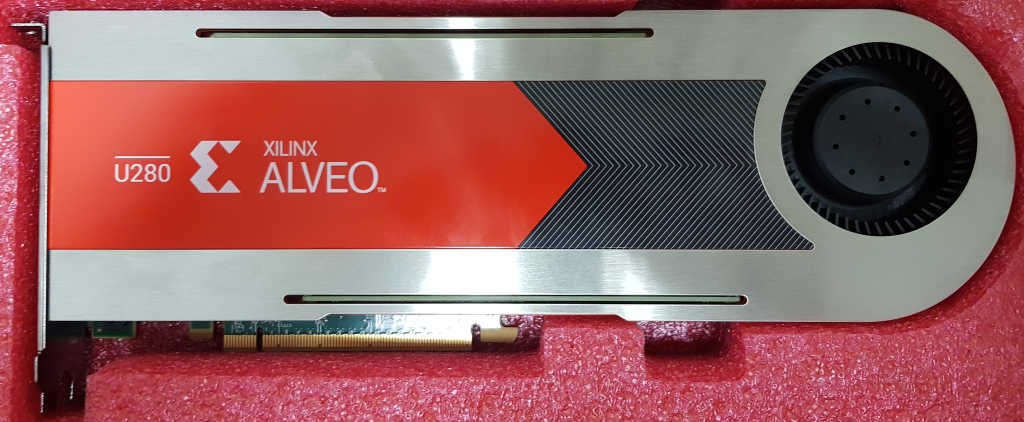
\includegraphics[width=\linewidth]{figures/U280.png}
    \caption{Xilinx U280实物图}
    \label{fig:U280}
\end{figure}



\section{软件与硬件性能评估}

基于上面生成的数据集,我们对我们的软件算法和硬件架构进行验证。对于软件算法而言,我们选择Python和C两种编程语言来实现基数排序、归并排序、堆排序等三种算法,通过Python和C语言标准库中的计时函数来测试完成排序的软件运行时间;对于硬件架构而言,我们使用Vitis HLS生成如表\ref{table:search_space}所示的13种硬件架构,并将其部署在U280加速卡上,测试其完成排序的总耗时,作为衡量硬件性能的标准。

\subsection{100万级别数据集性能测试}
将所有测试结果以柱状图形式绘出,如图\ref{fig:1MComparison}所示;
其中,详细的软件测试结果如表\ref{tab:1Msoftware}所示,详细硬件测试结果如表\ref{tab:1Mhardware}所示。
从上面的实验结果可以看出,在排序100万个数时,使用16进制基数排序+传统64路归并排序架构可以获得最好的性能,其仅需要10.72ms即可完成排序,相较于基于C语言最快的排序算法——16进制基数排序快了3.92倍;相较于基于Python语言最快的排序算法——堆排序快了96.08倍。

\begin{figure}[htbp]
    \centering
    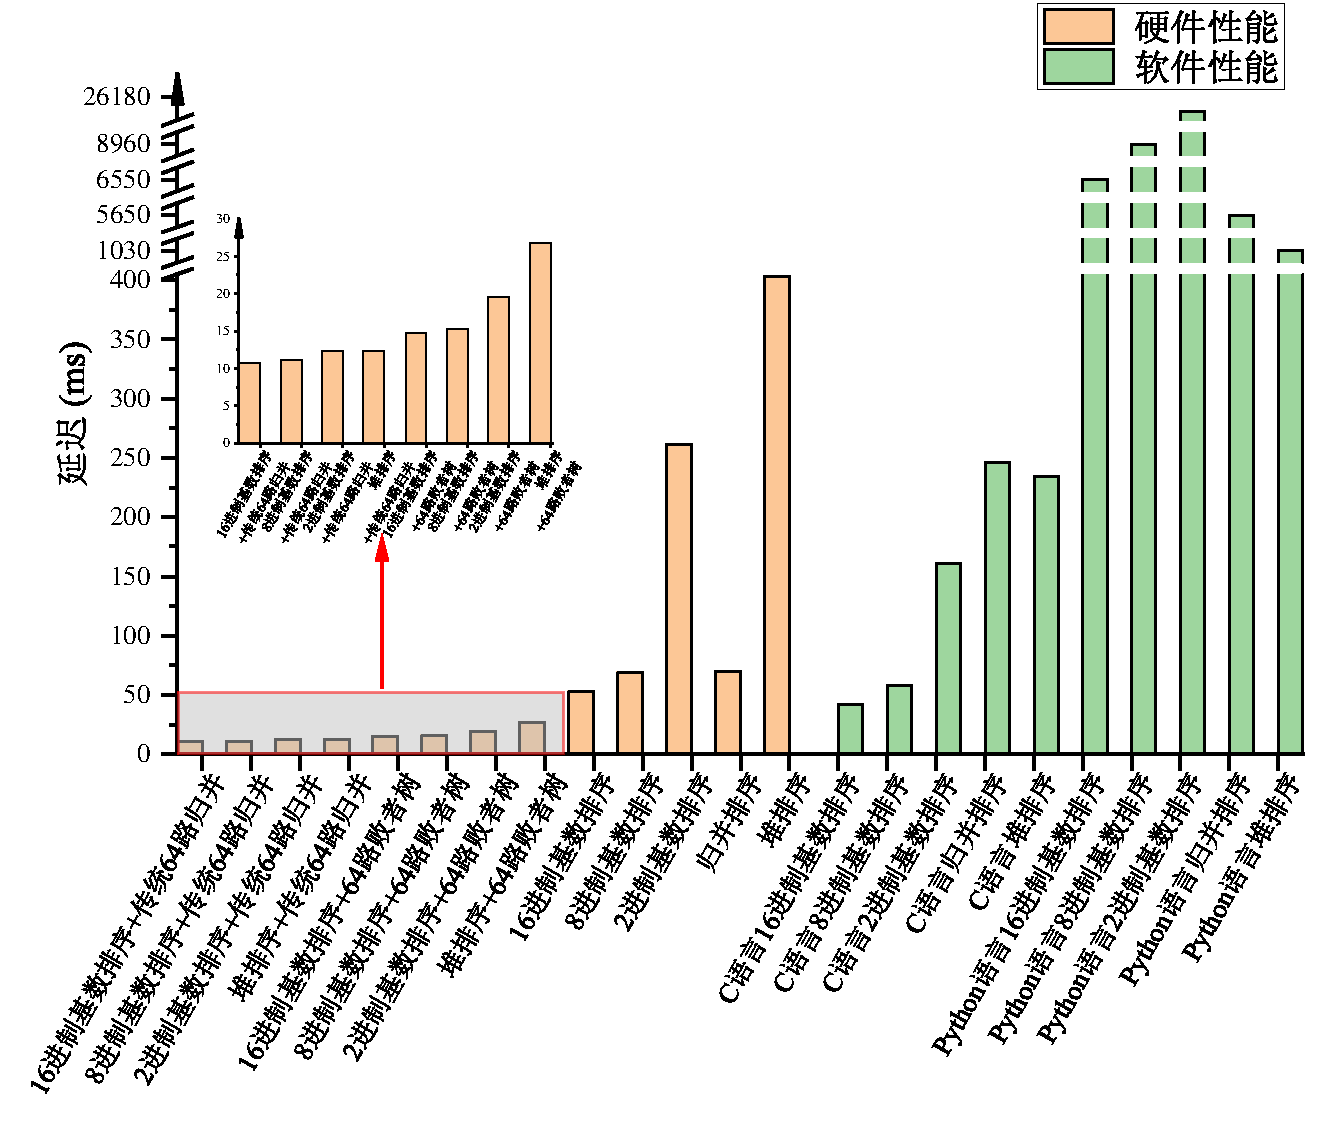
\includegraphics[width=\linewidth]{figures/1MComparison.pdf}
    \caption{100万数据集下不同平台性能对比}
    \label{fig:1MComparison}
\end{figure}


\begin{table}[htbp]
\centering
\caption{100万级别数据集软件性能测试}
\setlength{\tabcolsep}{10mm}{
\begin{tabular}{ccc}
\toprule
算法       & C语言耗时(ms) & Python语言耗时(ms) \\
\midrule
16进制基数排序 & \textbf{42}        & 6550           \\
8进制基数排序  & 58        & 8960           \\
2进制基数排序  & 161       & 26168          \\
归并排序     & 246       & 5650           \\
堆排序      & 234       & \textbf{1030}           \\
\bottomrule
\end{tabular}}
\label{tab:1Msoftware}
\end{table}



\begin{table}[htbp]
\caption{100万级别数据集硬件架构性能测试}
\resizebox{\linewidth}{!}{
\begin{tabular}{cccccccc}
\toprule
\multirow{2}{*}{硬件架构} & \multicolumn{4}{c}{硬件资源利用情况} & \multicolumn{3}{c}{性能}        \\
                      & BRAM & DSP & FF     & LUT    & 时钟周期      & 频率(MHz) & 总延迟(ms) \\
\midrule
16进制基数排序+传统64路归并      & 3040 & 128 & 162639 & 179055 & 2125245   & 198.26  & \textbf{10.72}   \\
8进制基数排序+传统64路归并       & 3040 & 128 & 99023  & 136431 & 2172099   & 194.74  & 11.15   \\
2进制基数排序+传统64路归并       & 3040 & 128 & 47183  & 117359 & 2500377   & 202.51  & 12.35   \\
堆排序+传统64路归并           & 2016 & 0   & 55823  & 114673 & 3074622   & 250     & 12.30   \\
16进制基数排序+64路败者树       & 2048 & 128 & 158447 & 164386 & 1156549   & 78.4    & 14.75   \\
8进制基数排序+64路败者树        & 2048 & 128 & 94831  & 121762 & 1203403   & 78.4    & 15.35   \\
2进制基数排序+64路败者树        & 2048 & 128 & 42991  & 102690 & 1531681   & 78.4    & 19.54   \\
堆排序+64路败者树            & 1024 & 0   & 51631  & 100004 & 2105931   & 78.4    & 26.86   \\
16进制基数排序              & 16   & 4   & 2424   & 2420   & 10000219  & 190.37  & 52.53   \\
8进制基数排序               & 16   & 4   & 1430   & 1748   & 13000195  & 190.37  & 68.29   \\
2进制基数排序               & 16   & 0   & 445    & 1327   & 65000452  & 248.63  & 261.43  \\
归并排序                  & 608  & 0   & 5420   & 14562  & 20000079  & 287.6   & 69.54   \\
堆排序                   & 0    & 0   & 803    & 1365   & 100740715 & 250     & 402.96 \\
\bottomrule
\end{tabular}}
\label{tab:1Mhardware}
\end{table}



\subsection{500万级别数据集性能测试}
类似上一节的做法,我们将所有测试结果以柱状图的形式给出,如图我们首先记录了软件性能测试结果和硬件测试结果,如图\ref{fig:5MComparison}所示。其中详细的软件测试结果和详细的硬件测试结果分别如表\ref{tab:5Msoftware}和表\ref{tab:5Mhardware}所示。

根据这些实验测得的数据,我们一样能够给出初步结论:在排序500万个数的时候,使用16进制基数排序+传统64路归并排序可以获得最好的性能,仅需53.83ms就可以完成排序,相较于基于C语言的最快算法——16进制基数排序快了4.12倍;相较于基于Python语言的最快排序算法——堆排序快了138.02倍。

\begin{figure}[htbp]
    \centering
    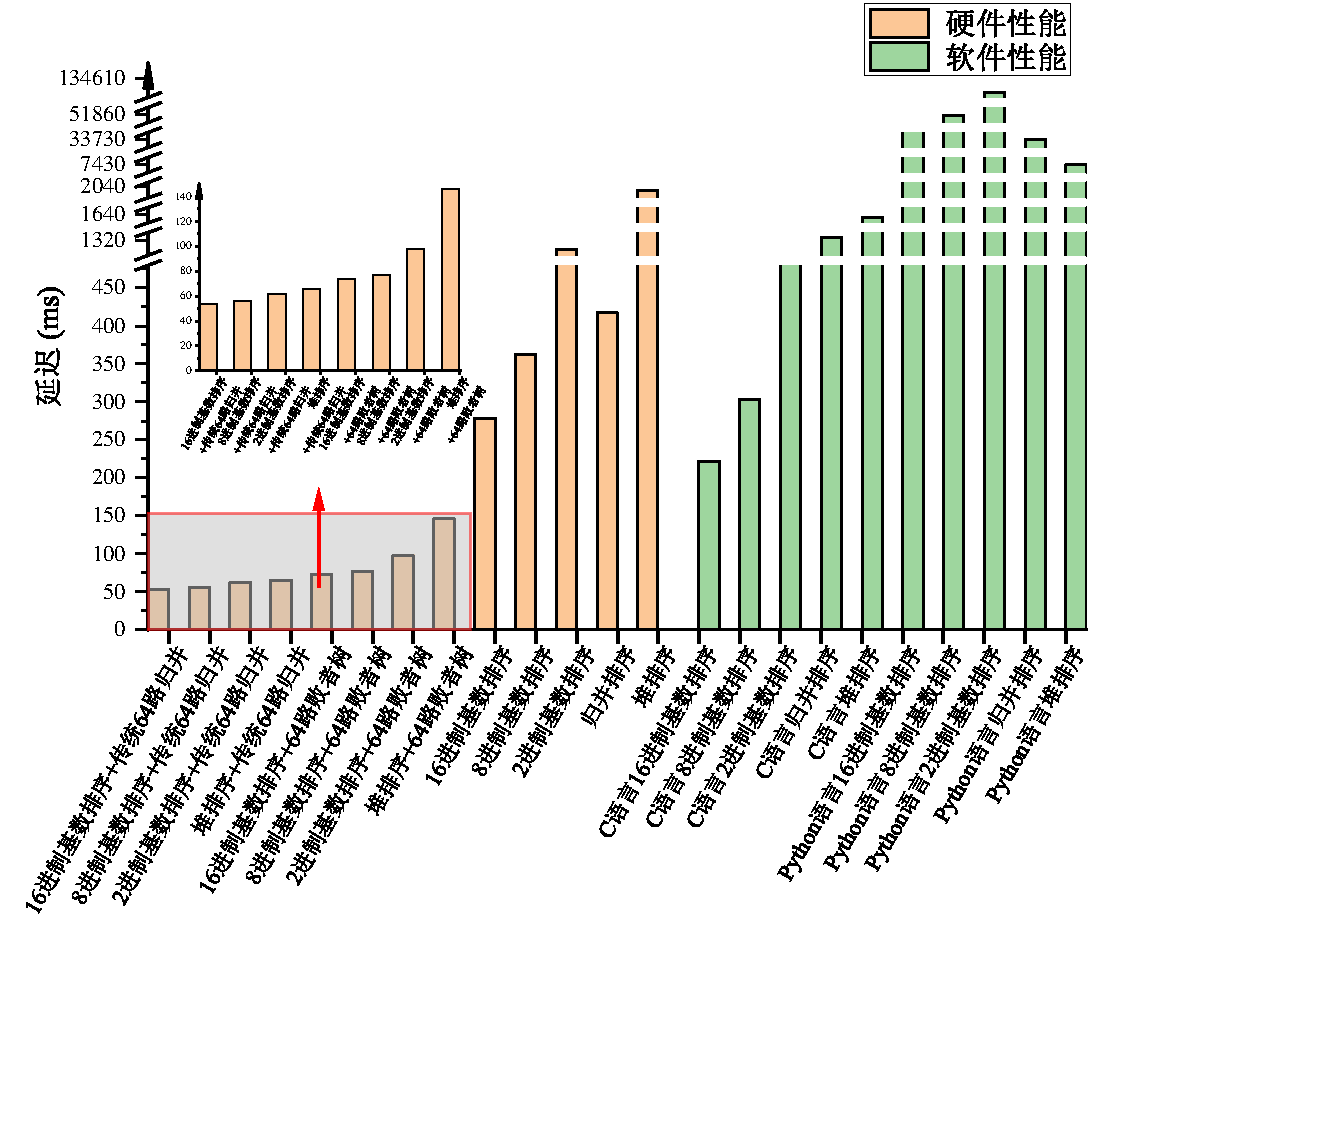
\includegraphics[width=\linewidth]{figures/5MComparison.pdf}
    \caption{500万数据集下不同平台性能对比}
    \label{fig:5MComparison}
\end{figure}


\begin{table}[htbp]
\centering
\caption{500万级别数据集软件性能测试}
\setlength{\tabcolsep}{10mm}{
\begin{tabular}{ccc}
\toprule
算法       & C语言耗时(ms) & Python语言耗时(ms) \\
\midrule
16进制基数排序 & \textbf{222}       & 34324          \\
8进制基数排序  & 303       & 51859          \\
2进制基数排序  & 795       & 134591         \\
归并排序     & 1323      & 33730          \\
堆排序      & 1637      & \textbf{7430}            \\
\bottomrule
\end{tabular}}
\label{tab:5Msoftware}
\end{table}


\begin{table}[htbp]
\centering
\caption{500万级别数据集硬件架构性能测试}
\resizebox{\linewidth}{!}{
\begin{tabular}{cccccccc}
\toprule
\multirow{2}{*}{硬件架构} & \multicolumn{4}{c}{硬件资源利用情况} & \multicolumn{3}{c}{性能}        \\
                      & BRAM & DSP & FF     & LUT    & 时钟周期      & 频率(MHz) & 总延迟(ms) \\
\midrule
16进制基数排序+传统64路归并      & 3040 & 128 & 164553 & 180848 & 10625245  & 197.39  & \textbf{53.83}   \\
8进制基数排序+传统64路归并       & 3040 & 128 & 100937 & 138032 & 10859599  & 193.91  & 56.00   \\
2进制基数排序+传统64路归并       & 3040 & 128 & 49097  & 119152 & 12500377  & 201.61  & 62.00   \\
堆排序+传统64路归并           & 2016 & 0   & 59273  & 116146 & 16283732  & 250     & 65.13   \\
16进制基数排序+64路败者树       & 2048 & 128 & 159986 & 165927 & 5781549   & 78.4    & 73.74   \\
8进制基数排序+64路败者树        & 2048 & 128 & 96370  & 123111 & 6015903   & 78.4    & 76.73   \\
2进制基数排序+64路败者树        & 2048 & 128 & 44530  & 104231 & 7656681   & 78.4    & 97.66   \\
堆排序+64路败者树            & 1024 & 0   & 54706  & 101225 & 11440041  & 78.4    & 145.92  \\
16进制基数排序              & 16   & 4   & 2448   & 2501   & 50000219  & 179.53  & 278.51  \\
8进制基数排序               & 16   & 4   & 1454   & 1826   & 65000195  & 179.53  & 362.06  \\
2进制基数排序               & 16   & 0   & 445    & 1327   & 325000452 & 248.63  & 1307.17 \\
归并排序                  & 736  & 0   & 6648   & 17594  & 120000095 & 287.6   & 417.25  \\
堆排序                   & 0    & 0   & 851    & 1387   & 508562774   & 250     &   2034.25      \\
\bottomrule
\end{tabular}}
\label{tab:5Mhardware}
\end{table}






\subsection{1000万级别数据集性能测试}

% 所有测试结果如图\ref{fig:10MComparison}所示,其中软件详细测试结果如表\ref{tab:10Msoftware}所示,硬件详细测试结果如图\ref{tab:10Mhardware}所示。

根据图\ref{fig:10MComparison}、表\ref{tab:10Msoftware}、表\ref{tab:10Mhardware}所示的数据,我们可以有如下结论:在对1000万数据进行排序的过程中,仍然是使用16进制基数排序+传统64路归并具有最好的性能,仅需107.78毫秒即可完成排序,相较于C语言最好的算法——16进制基数排序快了4.38倍;相较于Python语言最好的算法——堆排序快了163.48倍。

\begin{figure}[htbp]
    \centering
    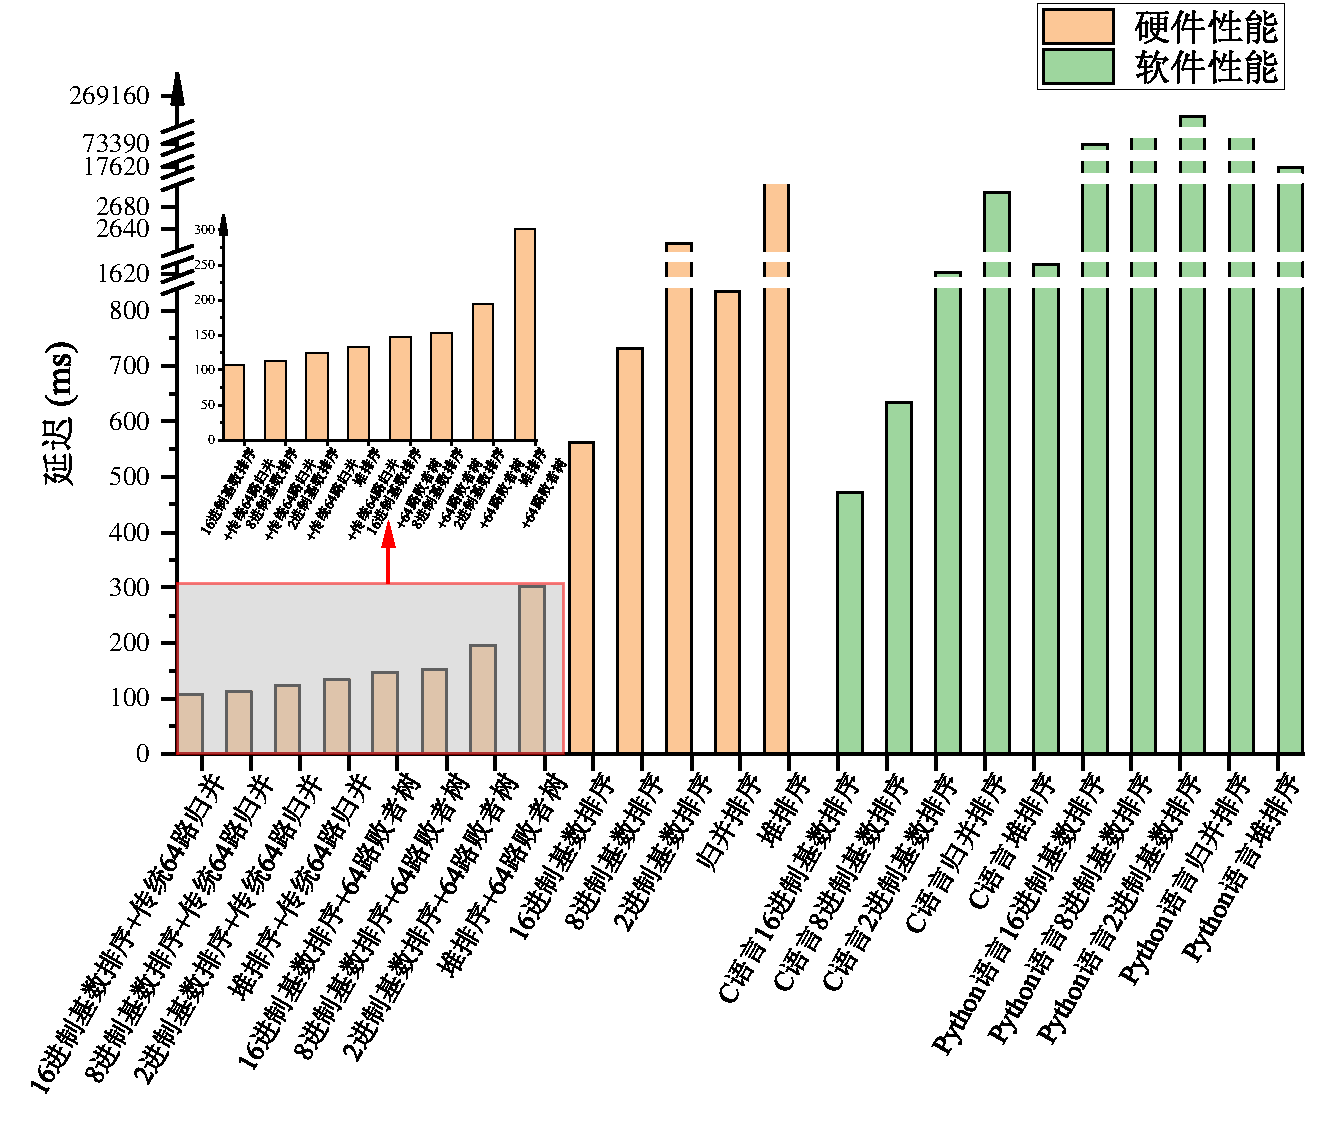
\includegraphics[width=\linewidth]{figures/10MComparison.pdf}
    \caption{1000万数据集下不同平台性能对比}
    \label{fig:10MComparison}
\end{figure}

\begin{table}[htbp]
\centering
\caption{1000万级别数据集软件性能测试}
\setlength{\tabcolsep}{10mm}{
\begin{tabular}{ccc}
\toprule
算法       & C语言耗时(ms) & Python语言耗时(ms) \\
\midrule
16进制基数排序 & \textbf{472}       & 73390          \\
8进制基数排序  & 634       & 97979          \\
2进制基数排序  & 1622      & 269123         \\
归并排序     & 2706      & 75360          \\
堆排序      & 1637      & \textbf{17620}      \\
\bottomrule
\end{tabular}}
\label{tab:10Msoftware}
\end{table}




% Please add the following required packages to your document preamble:
% \usepackage{multirow}
\begin{table}[htbp]
\centering
\caption{1000万级别数据集硬件架构性能测试}
\resizebox{\linewidth}{!}{
\begin{tabular}{cccccccc}
\toprule
\multirow{2}{*}{硬件架构} & \multicolumn{4}{c}{硬件资源利用情况} & \multicolumn{3}{c}{性能}        \\
                      & BRAM & DSP & FF     & LUT    & 时钟周期      & 频率(MHz) & 总延迟(ms) \\
\midrule
16进制基数排序+传统64路归并      & 3040 & 128 & 165191 & 180441 & 21250245  & 197.16  & \textbf{107.78}  \\
8进制基数排序+传统64路归并       & 3040 & 128 & 101575 & 138521 & 21718974  & 193.69  & 112.13  \\
2进制基数排序+传统64路归并       & 3040 & 128 & 49735  & 119705 & 25000377  & 201.37  & 124.15  \\
堆排序+传统64路归并           & 2016 & 0   & 60423  & 116635 & 33346887  & 250     & 133.39  \\
16进制基数排序+64路败者树       & 2048 & 128 & 160499 & 166376 & 11562799  & 78.4    & 147.48  \\
8进制基数排序+64路败者树        & 2048 & 128 & 96883  & 123496 & 12031528  & 78.4    & 153.46  \\
2进制基数排序+64路败者树        & 2048 & 128 & 45043  & 104680 & 15312931  & 78.4    & 195.32  \\
堆排序+64路败者树            & 1024 & 0   & 55731  & 101610 & 23659446  & 78.4    & 301.78  \\
16进制基数排序              & 16   & 4   & 2456   & 2528   & 100000219 & 177.75  & 562.59  \\
8进制基数排序               & 16   & 4   & 1462   & 1852   & 130000195 & 177.75  & 731.37  \\
2进制基数排序               & 16   & 0   & 450    & 1330   & 650000452 & 248.63  & 2614.33 \\
归并排序                  & 736  & 0   & 6696   & 17618  & 240000095 & 287.6   & 834.49  \\
堆排序                   & 0    & 0   & 867        & 1392       &  1018510822         & 250     & 4074.04    \\
\bottomrule
\end{tabular}}
\label{tab:10Mhardware}
\end{table}

\subsection{总结}
基于上述的实验结果,我们可以初步得出以下几个结论:
\begin{enumerate}
    \item 在常用的2进制、8进制、16进制基数排序当中,无论是软件算法还是硬件架构的实验结果都显示出16进制基数排序速度最快,8进制次之,2进制最慢。基于此我们可以推测其原因主要是对于16进制基数排序来说,其一次可以排序4个比特位,因此对于最外层循环来说(以32位整数为例),只需要8次循环即可完成排序。而与之对应的2进制基数排序则需要32次循环才能完成排序,因此16进制基数排序相对于2进制基数排序要更快;
    \item 使用多路混合排序架构的性能会优于单一排序算法的加速架构,其原因也是显然的:使用多路混合排序,能够大大提高排序过程的并行性,从而提升总体的性能;
    \item 在多路排序当中,我们使用了64路传统归并算法和64路败者树两种方法来对前序排序架构生成的64路有序数组进行排序。从实验结果我们可以看到相较于64路败者树,64路传统归并算法的优势更为明显。其延迟相对较低,且能够使FPGA以更高的频率工作。而从败者树归并的原理我们就可以发现,其过程难以去发掘潜在的并行性,且含有大量的比较和交换的过程,从而造成其整体的工作频率不高(仅有约78.4MHz),败者树的架构也限制了前序归并排序和堆排序的工作频率,造成整体效率偏低。
    \item 相较于Python,使用C语言编写的程序具有更加高的效率。其原因主要有以下几点:首先,Python是解释型语言,即在运行时需要通过解释器逐行解释并执行。而C语言是一种编译型语言,在运行之前,C代码会被编译器编译成机器码,因此在运行时不需要额外的解释过程。编译型语言通常比解释型语言更快,因为它们避免了运行时解释的开销;其次Python是一种动态类型的语言,这意味着变量在运行时才确定其类型。这增加了运行时的开销,因为解释器必须检查每个变量的类型并执行相应的操作。而C语言是静态类型语言,在编译时就确定了变量的类型,因此运行时无需进行类型检查,提高了执行效率;另外,Python的自动内存管理也会对性能造成一定损失;与此同时,C语言具有高度优化的编译器,可以生成高度优化的机器码,而Python的解释器在该方面的能力有限。
    \item 在上述三组实验当中,采用16进制基数排序+传统64路归并具有最高的硬件效率。相较于软件算法中最快的C语言16进制归并排序可以有4倍左右的提升;而相较于Python语言中最快的堆排序算法,则可以有最多近200倍的提升幅度。因此,我们可以认为,该架构是我们的硬件搜索空间当中性能最强的架构。在接下的一章中,我们将采用该架构来解决实际问题。
    \item 从三类不同大小的数据集测试数据中我们可以发现,硬件相对于软件的加速比是不断提升的:最优硬件架构“16进制基数排序+传统64路归并”相对于C语言16进制基数排序的加速比从100万数据时的3.92倍增长到1000万数据集时的4.38倍;相对于Python语言堆排序的加速比从100万数据时的138.02倍增长到163.48倍。这说明我们的硬件加速架构在数据集越大的时候越有优势,符合我们设计的初衷。
\end{enumerate}


